\section{Introduction}
\label{sec:intro}

Learned codecs now match or surpass the best standardized codecs in rate--distortion performance~\cite{balle2018,minnen2018,cheng2020,he2022elic,liu2023tcm,li2023dcvcdc,li2024dcvcfm}, and recent systems have turned that efficiency into real-time throughput~\cite{jia2025dcvcrt,li2026dcvcuf}.
Decoding, however, remains the expensive half of the pipeline.
In the intra codec of DCVC-UF~\cite{li2026dcvcuf}, a 1080p frame costs 454\,GMAC to synthesize, and 89\% of that is a stack of twelve identical blocks that every region of the frame passes through, whether it shows a textured crowd or a clear sky.
The bitstream already carries everything needed to reconstruct the easy regions early; the decoder simply has no way to stop.

Two lines of work address decoder cost, and both do so uniformly over the image.
Efficient codec design shrinks the synthesis transform once, for all content: lighter blocks~\cite{wang2023evc}, shallow decoders~\cite{yang2023shallow}, or width-switchable models~\cite{yang2021slimcae}.
Dynamic networks instead adapt computation to the input~\cite{han2022survey}, by exiting early~\cite{teerapittayanon2016,huang2018msdnet}, skipping blocks~\cite{wang2018skipnet,wu2018blockdrop,veit2018}, or dropping tokens~\cite{rao2021dynamicvit,yin2022avit}; but they decide per image, or they target recognition, where a wrong decision costs accuracy rather than visible artifacts.
The closest precedent is region-aware super-resolution~\cite{kong2021classsr,wang2022ape,jeong2024pcsr}, which routes each patch to a network of matching capacity.
These methods decode patches independently, so their savings come with seams, and they choose each patch's network at the decoder from the degraded input alone.

A codec is in a better position than either.
Its encoder sees the source image, so it can measure, not guess, how much quality each region loses at each depth, and it can send that decision to the decoder.
This is exactly how standardized codecs allocate effort: the encoder searches partitions and modes, and the decoder follows the signalled choice~\cite{sullivan2012hevc,bross2021vvc}.
Learned codecs have not used this freedom for decoder compute.

We present FLEX, a tile-wise early-exit decoder for DCVC-UF (\cref{fig:teaser}).
The frame is decoded by a shared full-frame stem, then cut into 256-pixel tiles, each of which leaves the remaining trunk at one of four exits; a lightweight adapter maps every exit to the input the released head expects.
Tiles are processed without halo in the trunk, and a grid seam repair module, costing 1.1\% of a decode, removes the boundary error before a shared full-frame head.
The encoder, the entropy model and the bitstream are unchanged, so the rate does not depend on the exits taken.
The exit map is chosen at the encoder by a per-frame search under a distortion budget and signalled in 43--67 bits on average, or predicted at the decoder by a router that needs only a per-frame scalar.

On 53 frames from the common test conditions (HEVC Classes B--E, UVG and MCL-JCV) at five quantization levels, FLEX removes 29.5\% of the decoder's multiply--accumulates at a mean loss of 0.087\,dB against the released decoder, and the decoder-side router retains 28.0\% (\cref{fig:intro_tradeoff}).
Content-blind allocations with the same budget, one exit for the whole frame or an ordered dither of two exits, recover 21.1\% and 25.4\%.
The saving is realized in wall-clock time: at 1080p the routed decoder runs in 86\% of the released decoder's time.

Our contributions are:
\begin{itemize}
\item a tile-wise early-exit ladder for the synthesis transform of a state-of-the-art neural codec, trained through the tiled path it is deployed on, that leaves the encoder and bitstream of the released model untouched;
\item a grid seam repair module that makes independent, halo-free tiles viable at a cost of 1.1\% of a decode;
\item encoder-side exit selection signalled as side information, and a decoder-side router, compared against content-blind allocations to isolate the value of adapting to content;
\item an evaluation on real bitstreams and real tiled decodes, including wall-clock time and encoder overhead.
\end{itemize}

\begin{figure}[t]
\centering
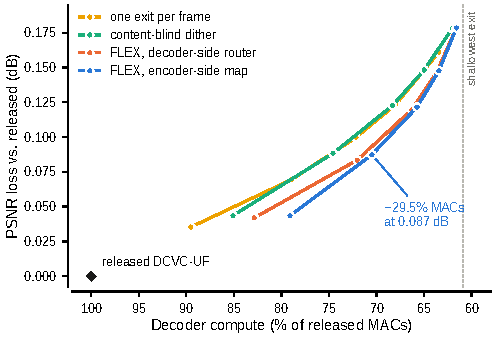
\includegraphics[width=\linewidth]{figs/intro_tradeoff.pdf}
\caption{\textbf{Decoder compute against quality} for DCVC-UF on 53 CTC frames at five QPs. Points are distortion budgets from 0.05 to 0.3\,dB.}
\label{fig:intro_tradeoff}
\end{figure}
